\scanpage{147}
\deleted{Si on a choisi les $\bar s''$ et $\bar s'$ tels que \unsure{$\operatorname{diag}$} \inserted{\unsure{$s''=\operatorname{diag}_2(\bar s')$|$s'''=\operatorname{diag}_{\theta_2}(s'')$}} et \unsure{$s'''=\operatorname{diag}_3(\bar s')$|$s'''=\operatorname{diag}_{g_3}(s')$} \unsure{diag.|donc}.}

Il est loisible de supposer que pour \unsure{tt|$\forall$} $s'\in E'$, désignant par $s''$ et $s'''$ ses images dans $\unsure{E''',E'''|E'',E'''}$ par l'application diagonale, \deleted{on ait $\bar s''=\mathrm{diag}$.} $\unsure{\widetilde{\bar s}''|\bar s'''}$ sont les images de $\underline{\bar s'}$ et $\underline{\bar s''}$ par les morphismes diagonaux, et qu'on ait choisi \inserted{pour} les données \unsure{classes de chemins,|chemins de chemins,} \unsure{associées|associés} à ces $s'',s'''$ \deleted{les} les chemins triviaux. \inserted{(\unsure{Enfin}, on peut supp. que $s''=\bar s'$.)} Alors il résulte de $c$ qu'on a

\[
g_{s''}=g_{s''}g_{s''}\qquad\text{i.e.}\quad g_{s''}=1
\]

et \unsure{la relation|les relations} b) \unsure{prend|prennent|pour} la forme équivalente

\[
\tag*{b')}g_{\bar s'}=1.
\]

\figure{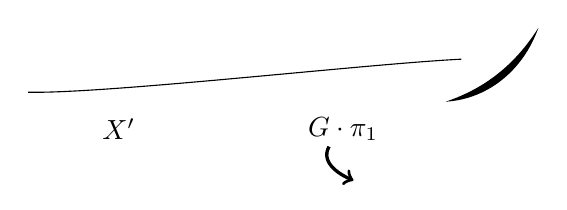
\begin{tikzpicture}[x=1cm,y=1cm]
\draw (0,0) .. controls (1,-.02) and (4.3,.36) .. (5.5,.42);
\fill (5.3,-.12) .. controls (5.75,.03) and (6.16,.31) .. (6.48,.82) .. controls (6.28,.26) and (5.82,-.09) .. (5.3,-.12);
\node at (1.15,-.47) {$X'$}; \node at (4,-.47) {$G\mathbin{\cdot}\pi_1$};
\draw[->,very thick] (3.82,-.69) .. controls (3.7,-.91) and (3.99,-1.06) .. (4.13,-1.12);
\end{tikzpicture}}

\[
S\longleftarrow S'
\]

\[
\begin{aligned}
&\pi\\[-2pt]
&\qquad\pi_1(\unsure{s'_1,a'|S',a'|S,\alpha})\quad\pi\qquad S
\end{aligned}
\]

\diagram{\begin{tikzcd}[ampersand replacement=\&,column sep=small]
\&R_0\arrow[d]\&R_1\arrow[d]\&R_2\arrow[d,shift left]\arrow[d]\arrow[d,shift right]\\
S\&S'\arrow[l]\&S''\arrow[l,shift left]\arrow[l,shift right]\&S'''\arrow[l,shift left=2]\arrow[l]\arrow[l,shift right=2]
\end{tikzcd}}

% archive sheet number: 146

